\section{The Five Graph Archetypes}\label{sec:archetypes}

The experimental catalog reveals five fundamental graph topologies, each with a distinct physical interpretation. These are not postulated---they emerge directly from the Killing spectrum.

\subsection{Archetype I: Pure Cycle Graph---$\Kil \propto -I$}\label{sec:archetype_I}

\textbf{Signature:} $(0^+, 0_0, n^-)$

\textbf{Examples:} All compact simple algebras (SU(N), SO(N), Sp(2N), G$_2$, F$_4$, E$_6$)

\begin{figure}[h]
\centering
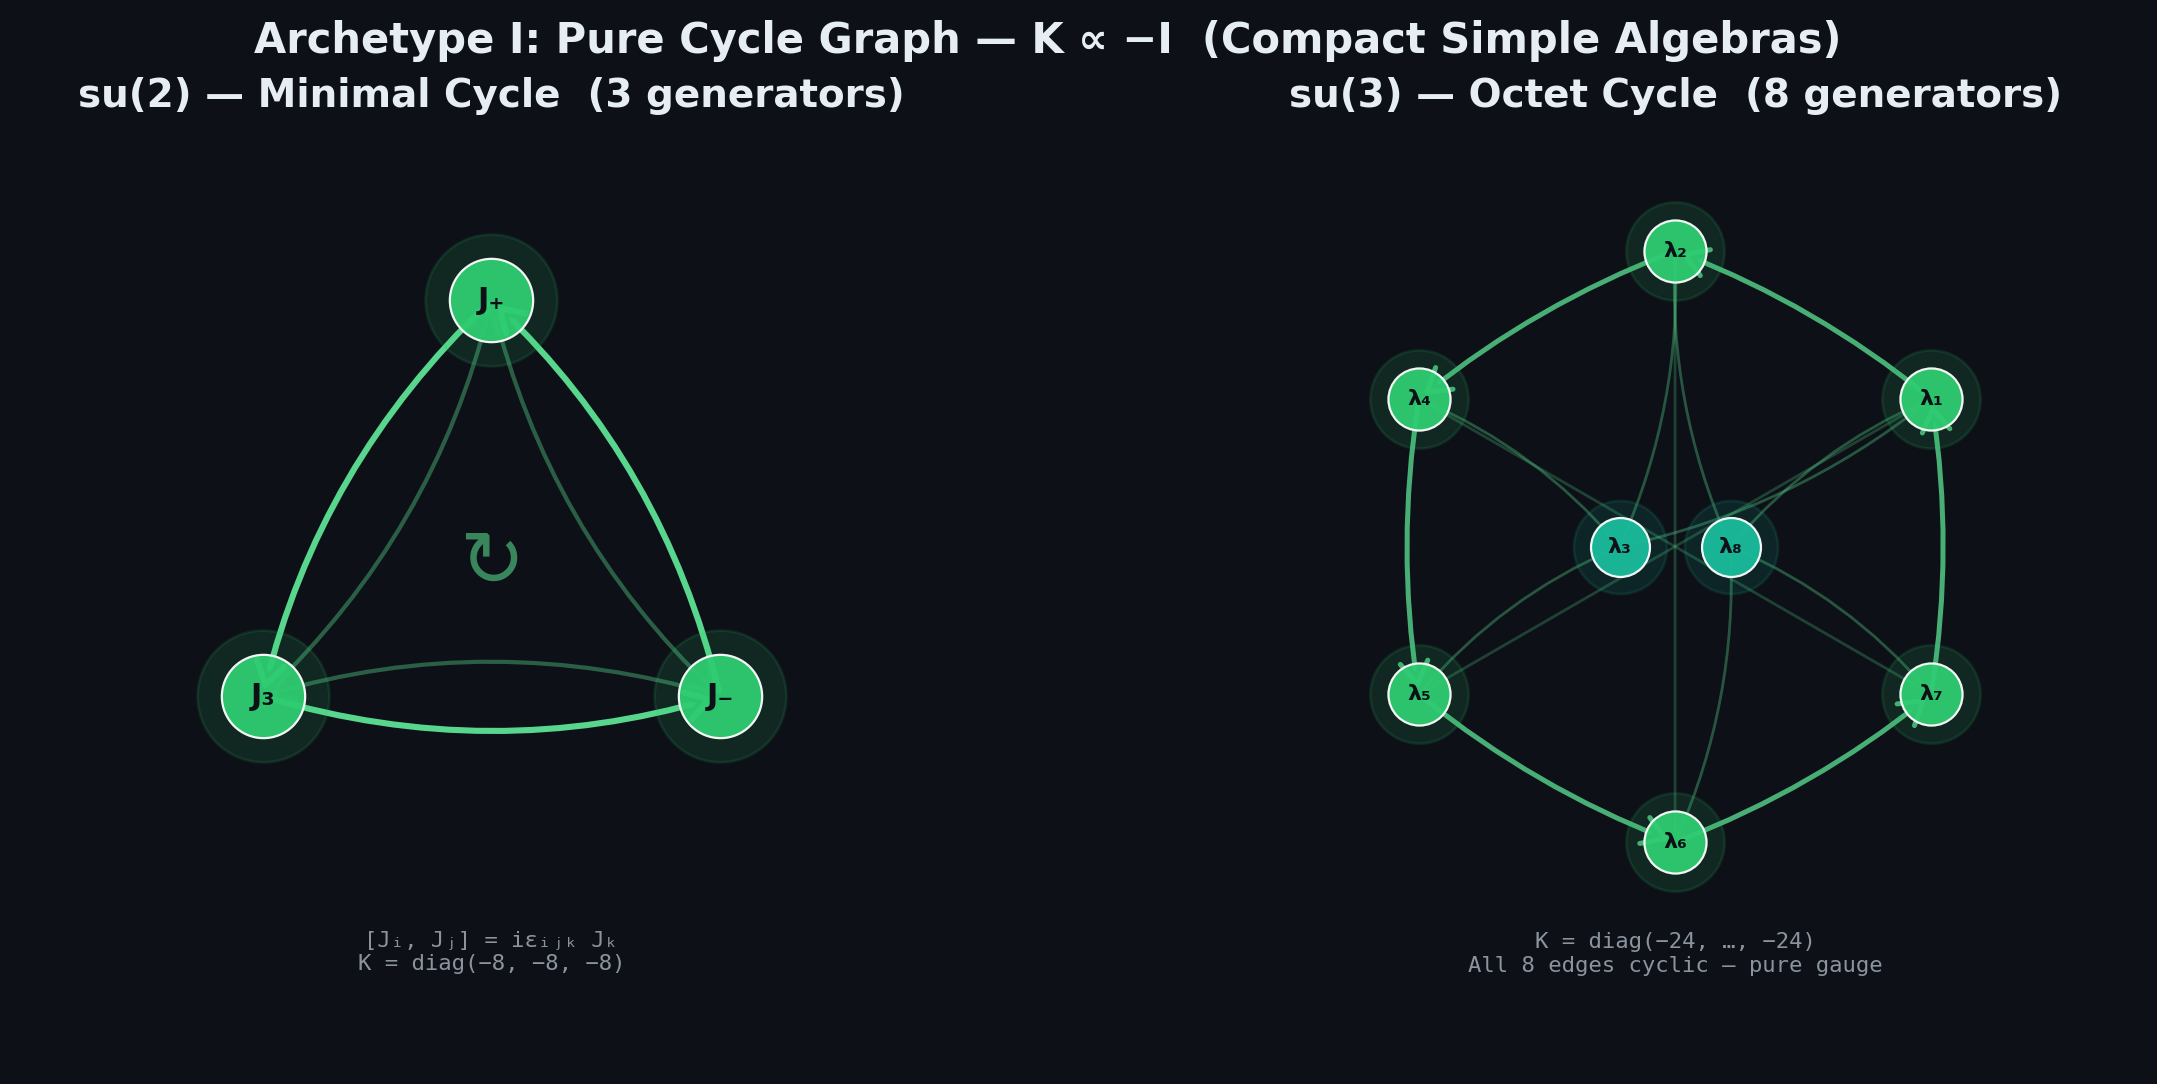
\includegraphics[width=0.8\textwidth]{figures/fig2_archetype_I_pure_cycle.png}
\caption{Archetype I: su(2) minimal triangle and su(3) octet cycle. Every edge participates in at least one closed cycle via the adjoint action.}
\end{figure}

\paragraph{Structure.} Every edge participates in at least one closed cycle via the adjoint action. The graph has no open ends, no dangling strands. All generators feed back onto themselves through commutators. The graph is \emph{homogeneous}: no edge is more central or more peripheral than any other.

\paragraph{Physical interpretation.} Internal gauge symmetries. The cyclic structure means every gauge transformation can be undone---applying $e^{i\theta T_a}$ followed by $e^{-i\theta T_a}$ returns to the identity. The group manifold is compact.

\paragraph{Graph properties:}
\begin{itemize}
    \item All loops are contractible (simply connected for SU(N))
    \item The number of independent cycles equals $\dim(\g)$
    \item Holonomy $U_\circlearrowleft = \exp(i \oint A) \neq I$ encodes the physical content
    \item Density threshold: $\ro = n_{\mathrm{gen}} / (d^2 - 1) = 1$ (all $n$ edges required; removing any one collapses the entire cycle structure)
\end{itemize}

\paragraph{Why all eigenvalues are equal.} For simple compact algebras, the Killing form is proportional to the identity ($\Kil = -h^\vee \cdot g$). This means all cycles have the same ``strength''---every edge participates equally in the adjoint feedback network. In graph terms: the graph is \emph{homogeneous}. This is the algebraic expression of gauge democracy.

\paragraph{Minimal example---$\su(2)$ (3 generators):}Minimal cycle: 3 edges, 1 independent loop. Every commutator $[J_i, J_j] = i\epsilon_{ijk} J_k$ closes within the triangle. The graph is the complete graph $K_3$.

\paragraph{Complex example---$\su(3)$ (8 generators):}8 edges, multiple interlocking cycles. The Cartan subalgebra ($\lambda_3, \lambda_8$) forms a 2D torus of diagonal generators; the remaining 6 are root vectors forming hexagonal cycles. The graph is NOT the complete graph---some commutators vanish (like $[\lambda_3, \lambda_8] = 0$), so some edges are not directly connected.

\subsection{Archetype II: Mixed Graph---$(p^+, q^-)$}\label{sec:archetype_II}

\textbf{Signature:} $(p^+, q^-)$, no zero eigenvalues

\textbf{Examples:} $\slg(2,\R)$ (1+, 2$-$), $\so(3,1)$ (3+, 3$-$), $\su(2,2)$ (8+, 7$-$)

\begin{figure}[h]
\centering
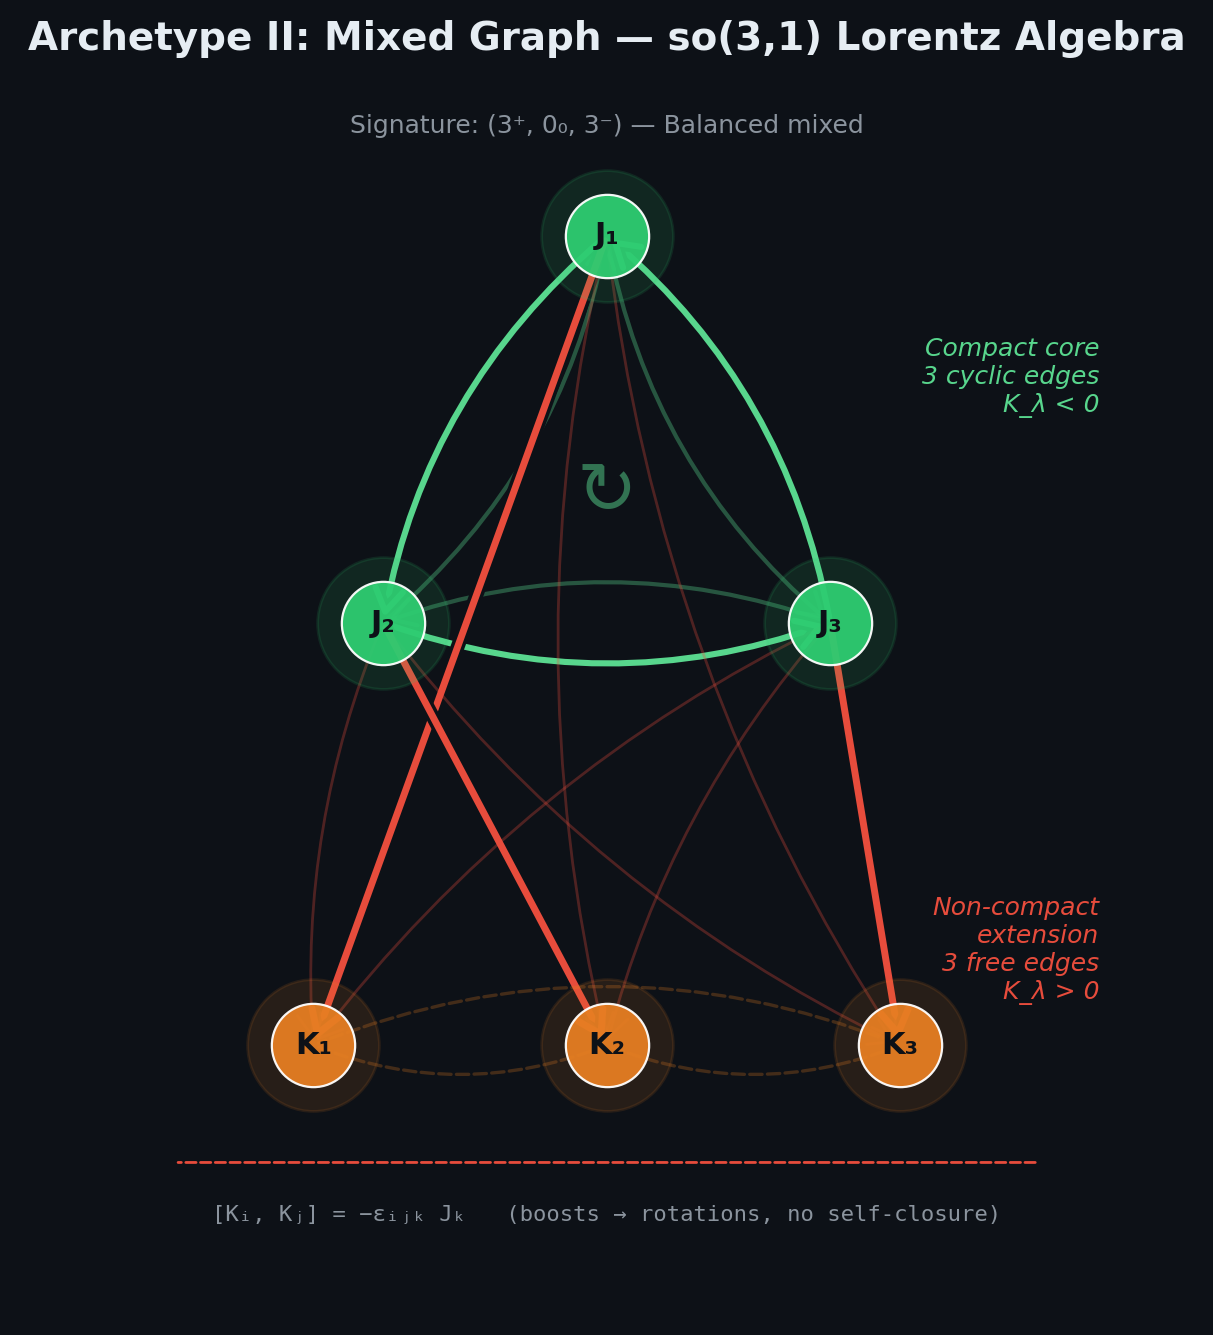
\includegraphics[width=0.8\textwidth]{figures/fig3_archetype_II_mixed_lorentz.png}
\caption{Archetype II: so(3,1) Lorentz algebra with rotation core and boost extensions. Signature $(3^+, 3^-)$---balanced mixed.}
\end{figure}

\paragraph{Structure.} The graph has a \textbf{compact core} of $q$ cyclic edges plus $p$ \textbf{open extensions} that emerge from the core but do not close back. The cyclic core forms the maximal compact subalgebra; the free extensions are the non-compact coset directions.

\paragraph{Physical interpretation.} Spacetime symmetries. The compact core carries rotations (undoable); the open extensions carry boosts (irreversible mixing of space and time) or translations (displacements).

\paragraph{Concrete example---$\so(3,1)$:}Rotation generators \{$J_1, J_2, J_3$\} form a closed $\so(3)$ cycle: $[J_i, J_j] = \epsilon_{ijk} J_k$. Boost generators  \{$K_1, K_2, K_3$\} extend outward: $[K_i, K_j] = -\epsilon_{ijk} J_k$ (commuting two boosts gives a rotation---the free edges connect back to the core but do not form their own cycle).

The free (boost) edges are \textbf{not independent}---they are \emph{driven by} the cyclic core. Removing the rotations would leave the boosts unable to close among themselves. The graph has a hierarchical structure: \textbf{compact core $\to$ non-compact extension}.

\paragraph{Concrete example---$\su(2,2)$ (conformal algebra):}7 compact edges (maximal compact $\mathfrak{s}(\mathfrak{u}(2) \oplus \mathfrak{u}(2)))$ plus 8 free edges (translations, special conformal, dilatation, boosts). The 8 $>$ 7 free-to-cycle ratio reflects the fact that conformal symmetry has more spacetime directions than internal directions.

\paragraph{The frustration experiment.} When compact Killing target is imposed on $\et$-preserving generators, the optimizer \emph{kills the boost edges} (forces $\Kil_{\mathrm{boost}} \to 0$), recovering the compact core $\so(3)$. The free extensions collapse.

\subsection{Archetype III: Cycle + Strand---$(0^+, k_0, n^-)$}\label{sec:archetype_III}

\textbf{Signature:} $k > 0$ zero eigenvalues, $n > 0$ negative eigenvalues

\textbf{Examples:} $\fu(2)$ (0+, 1$_0$, 3$-$), $\fu(3)$ (0+, 1$_0$, 8$-$)

\begin{figure}[h]
\centering
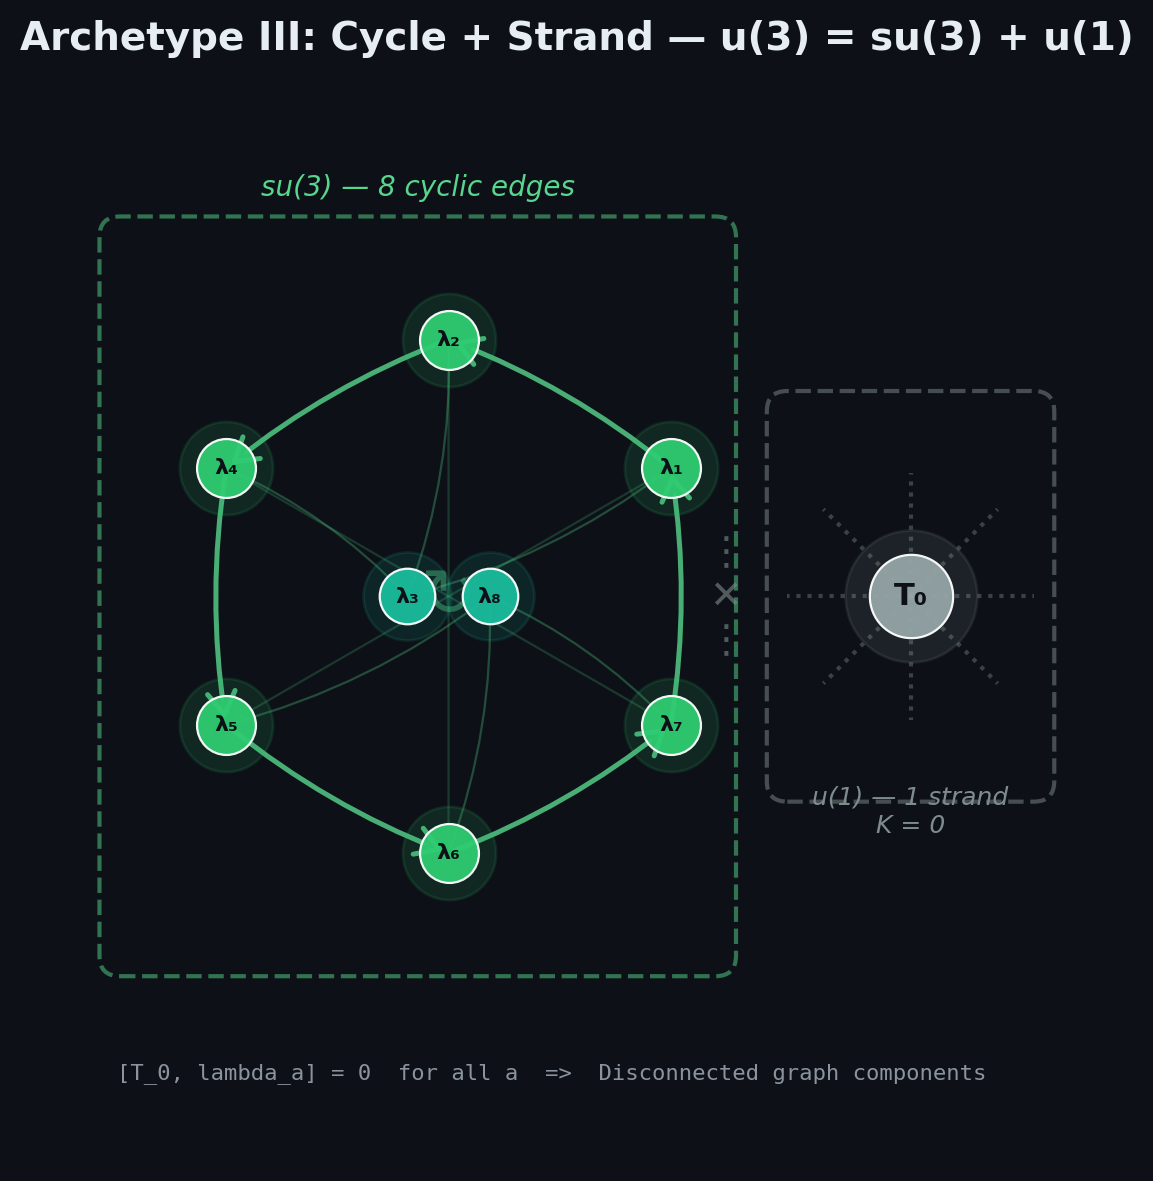
\includegraphics[width=0.8\textwidth]{figures/fig5_archetype_III_cycle_strand.png}
\caption{Archetype III: u(3) = su(3) cycle + u(1) decoupled strand. The abelian generator $T_0$ satisfies $[T_0, T_a] = 0$ for all $a$, so $\Kil_{0a} = 0$ for all $a$.}
\end{figure}

\paragraph{Structure.} The graph has a \textbf{compact cyclic core} (the semisimple part) plus one or more \textbf{disconnected strands} (the abelian factor). The strands are not connected to the core by any edges---they float independently in the graph.

\paragraph{Physical interpretation.} The cyclic core carries the non-abelian gauge symmetry; the decoupled strand carries the U(1) phase. The electromagnetic field $A_\mu$ lives on the strand; the gluon fields $G_\mu^a$ live on the core.

\paragraph{Why the strand is decoupled.} The abelian generator $T_0$ satisfies $[T_0, T_a] = 0$ for all $a$, so $\Kil_{0a} = 0$ for all $a$. It has zero adjoint feedback---it doesn't participate in any cycle. Every other generator ignores it.

\paragraph{Graph property.} This is the only archetype where the graph is \textbf{disconnected}. The removal of the strand does not affect the core, and vice versa. In physical terms: U(1)$_{\mathrm{EM}}$ does not mix with SU(3)$_{\mathrm{color}}$ at tree level.

\paragraph{The U(3) experiment.} In $\fu(3)$, the Killing matrix has exactly 1 zero eigenvalue and 8 degenerate negative eigenvalues at $-0.950$. The zero-eigenvalue eigenvector is proportional to $I_{3\times 3}$---the identity matrix, which commutes with everything. The $8 + 1$ decomposition $\fu(3) = \su(3) \oplus \fu(1)$ is visible directly in the graph: 8 interlocking cycles + 1 isolated strand.

\subsection{Archetype IV: Pure Free Graph---$(n^+, 0_0, 0^-)$}\label{sec:archetype_IV}

\textbf{Signature:} All positive eigenvalues

\textbf{Status:} Not yet observed experimentally---would require a non-compact algebra with no compact subalgebra.

\paragraph{Theoretical status.} This would correspond to a purely non-compact ``algebra'' with no internal rotations---all degrees of freedom are causal/translational. The Poincar\'e algebra's translation sector $\{P_\mu\}$ has this structure locally (abelian sub-sector), but the full Poincar\'e algebra includes rotations and is mixed.

\paragraph{Physical speculation.} A purely free graph might correspond to a region of the evolution graph with no gauge symmetry at all---pure free evolution, no feedback, no cycles. In the SS-PEG framework, this is the $\ro < 1$ regime: \textbf{pre-crystallization}, where relational density is too low for any symmetry to form.

\subsection{Archetype V: Frustrated/Degenerate Graph---$(0^+, k_0, q^-)$ with $k \gg 1$}\label{sec:archetype_V}

\textbf{Signature:} Many zero eigenvalues alongside negative eigenvalues

\textbf{Examples:} so(3,1) frustrated $\to$ so(3) + 3 degenerate; su(2,2) frustrated $\to$ 9 compact + 6 degenerate

\paragraph{Structure.} The graph has a \textbf{reduced cyclic core} (the maximal compact subalgebra) plus several \textbf{collapsed strands}---generators that were forced out of the algebra by an incompatible constraint. Unlike Archetype III, these strands are not physically meaningful---they are artifacts of frustration.

\paragraph{Physical interpretation.} This is what happens when you try to force a non-compact algebra into a compact box. The graph cannot support the full algebra, so it sheds the non-compact edges. The surviving compact core is the \textbf{maximal compact subalgebra}:
\begin{itemize}
    \item $\so(3,1)$ frustrated $\to$ $\so(3)$ (rotations survive, boosts collapse)
    \item $\su(2,2)$ frustrated $\to$ $\mathfrak{s}(\mathfrak{u}(2) \oplus \mathfrak{u}(2))$ (9D compact part survives, 6 non-compact collapse)
\end{itemize}

\paragraph{Physical analogy.} This is like cooling a liquid crystal into its ordered phase---the orientational degrees of freedom that can't fit the crystal symmetry are quenched out. The graph reveals which edges are ``compatible with compactness'' and which are not.

\subsection{Summary Table of Archetypes}\label{sec:archetype_summary}

\begin{table}[h]
\centering
\begin{tabular}{c c c c c c c}
\hline\hline
Archetype & Signature & Examples & Compact core & Free edges & Decoupled & Graph type \\
\hline
I & $(0^+, 0_0, n^-)$ & SU, SO, Sp, G$_2$, F$_4$, E$_6$ & $n$ & 0 & 0 & Connected, cyclic \\
II & $(p^+, q^-)$ & sl(2,$\R$), so(3,1), su(2,2) & $q$ & $p$ & 0 & Connected, mixed \\
III & $(0^+, k_0, n^-)$ & U(2), U(3) & $n$ & 0 & $k$ & Disconnected \\
IV & $(n^+, 0_0, 0^-)$ & --- & 0 & $n$ & 0 & All open \\
V & $(0^+, k_0, q^-)$ & so(3,1) frust., su(2,2) frust. & $q$ & 0 & $k$ & Reduced + degenerate \\
\hline\hline
\end{tabular}
\caption{Summary of the five graph archetypes.}
\end{table}
